\documentclass{beamer}
\usepackage{beamerthemesplit}
\usepackage{graphicx}

\usetheme{Madrid}

\usepackage{amsmath}
\usepackage[russian]{babel}

\title[Supportive MSSA]{Поддерживающие временные ряды в MSSA}
\subtitle{(продолжение)}
\author[Егор Ткаченко]{Ткаченко Егор Андреевич, группа 19.Б04}
\date[21.12.2021]{21 декабря 2021г.}
\logo{
\includegraphics[width=1cm]{logo.jpg}}
\institute[]{Санкт-Петербургский государственный университет\\Прикладная математика и информатика\\Кафедра статистического моделирования\\Научный руководитель: к.ф.-м.н., доцент Голяндина Н.Э.}

\begin{document}
    \begin{frame}
        \titlepage
    \end{frame}
    
    \begin{frame}
        \frametitle{Базовые определения}
        \begin{block}{Временной ряд}
            Вещественный временной ряд длины $N_p$:
            $$\mathsf{F}_p = (f^{(p)}_0, \dots, f^{(p)}_{N_p - 1}), f^{(p)}_j \in \mathbb{R}.$$
        \end{block}

        

        \begin{block}{Многомерный временной ряд}
            Многомерный временной ряд $\mathsf{F}$ --- набор $s$ временных рядов $\mathsf{F}_p$ длин~$N_p$:
            $$\{\mathsf{F}_p, p=1, \dots, s\}$$
        \end{block}
    \end{frame}

    \begin{frame}
        \frametitle{Определения}
        \begin{block}{Траекторная матрица}
            $L$-Траекторная матрица ряда $\mathsf{F}_p$:
            $$\mathcal{T}_{SSA}(\mathsf{F}_p) =
            \begin{pmatrix}
                f^{(p)}_0     & f^{(p)}_1 & \dots  & f^{(p)}_{K-1}\\
                f^{(p)}_1     & f^{(p)}_2 & \dots  & f^{(p)}_K\\
                \vdots        & \vdots    & \ddots & \vdots\\
                f^{(p)}_{L-1} & f^{(p)}_L & \dots  & f^{(p)}_{N_p-1}\\
            \end{pmatrix};$$
            для многомерного ряда $\mathsf{F}$:\quad
            $\mathcal{T}_{MSSA}(\mathsf{F}) = [\mathcal{T}_{SSA}(\mathsf{F}_1): \dotso :\mathcal{T}_{SSA}(\mathsf{F}_s)].$\\
            Из траекторной матрицы можно восстановить ряд.

        \end{block}

        \begin{block}{Ранг}
            Ранг ряда $\mathsf{F_p}$ (многомерного ряда $\mathsf{F}$) --- это ранг его траекторной матрицы: $r_p = \mathsf{rank}\ \mathcal{T}_{SSA}(\mathsf{F_p})$\quad ($r_{MSSA} = \mathsf{rank}\ \mathcal{T}_{MSSA}(\mathsf{F})$)
        \end{block}
    \end{frame}

    \begin{frame}
        \frametitle{Применение SSA и MSSA}
        \structure{\textbf{Вход:}}
        Ряд $\mathsf{F_1}$ для SSA или многомерный ряд $\mathsf{F}$ для MSSA;\\
        длина окна $L \leq N_1$ для SSA или $L \leq N_p$ для MSSA;\\
        ранг аппроксимирующего ряда r.\\
        
        \begin{block}{Алгоритм}
            \begin{enumerate}
                \item[1] Получение L-траекторной матрицы $\mathbf{X}$ временного ряда:\\
                    $\mathbf{X} = \mathcal{T}_{SSA}(\mathsf{F_1})$ для SSA или $\mathbf{X} = \mathcal{T}_{MSSA}(\mathsf{F})$ для MSSA.
                \item[2] Методом SVD матрица $\mathbf{X}$ раскладывается на сумму $d$ матриц $\mathbf{X}_i$ ранга 1, где: $d = \mathsf{rank}\ \mathbf{X}$.
                % $\mathbf{X}_i = \sqrt{\lambda_i}U_iV_i^T$, где: $d = \mathsf{rank}\ \mathbf{X}$;\\
                % $\lambda_i$ --- собственные числа матрицы $\mathbf{XX}^T$ ($\lambda_1 \geq \dotso \geq \lambda_L \geq 0$);\\
                % $U_i$ --- собственные вектора матрицы $\mathbf{XX}^T$; $V_i = \mathbf{X}^T U_i / \sqrt{\lambda_i}$.\\
                \item[3] Первые $r$ матриц $\mathbf{X}_i$ складываются и восстанавливаются в ряд (SSA) или многомерный ряд (MSSA)
            \end{enumerate}
        \end{block}
        
        \structure{\textbf{Выход:}}
        Аппроксимирующий ряд конечного ранга r.
    \end{frame}

    \begin{frame}
        \begin{block}{Линейная рекуррентная формула; управляемый ЛРФ ряд}
            % ЛРФ --- формула, выражающая каждый член последовательности через линейную комбинацию предыдущих членов.\\
            Ряд $\mathsf{F_p} = (f_i)_{i=0}^{N_p-1}$ --- управляемый ЛРФ, если существуют такие $a_1, \dotso, a_d$, что:
            $$f_{i+d} = \sum_{k=1}^d a_k f_{i+d-k},\ 0 \leq i \leq N_p - 1 - d,\ a_d \neq 0,\ t < N_p - 1.$$
        \end{block}

        \begin{block}{Замечание}
            Ряд конечного ранга является управляемым ЛРФ.
        \end{block}
        
        \begin{block}{Прогноз ряда}
            Прогноз вещественного временного ряда $\mathsf{F}_p$:
            $$\overset{\sim}{\mathsf{f}}_{N_p} = \sum_{k=1}^{L-1} a_k f_{N_p-k}.$$
            % $$\overset{\sim}{\mathsf{f}}_{N_p} = (\overset{\sim}{f}_{N_p}, \dots, \overset{\sim}{f}_{N_p + \overset{\sim}{N}_p - 1}), \overset{\sim}{f_j} \in \mathbb{R}.$$
        \end{block}

        % \begin{block}{Коэффициенты ЛРФ $a_1, \dotso, a_{L-1}$}
        %     $$(a_1, \dotso, a_{L-1}) = \mathcal{R}_L=\frac{1}{1-\sum_{j=1}^r \pi(U_j)^2} \sum_{j=1}^r \pi(U_j) \underline{U_j},$$
        %     где $\pi(U_j)$ --- последняя координата вектора $U_j$,\\ $\underline{U_j}$ --- вектор $U_j$ без последней координаты.
        % \end{block}
    \end{frame}

    \begin{frame}
        \frametitle{Задача}

        Пусть имеется временной ряд $\mathsf{F_1 = S_1 + R_1}$, где
        \begin{itemize}
            \item Сигнал $\mathsf{S_1}$ --- ряд управляемый ЛРФ.
            \item Шум $\mathsf{R_1}$ --- ряд без структуры.
        \end{itemize} 

        \structure{\textbf{Задача:}}
        спрогнозировать сигнал $\mathsf{S_1}$.

        Пусть помимо ряда $\mathsf{F_1}$ имеется временной ряд $\mathsf{F_2}$.

        \structure{\textbf{Идея:}}
        использование ряда $\mathsf{F_2}$ может улучшить прогноз сигнала $\mathsf{S_1}$.

        \begin{itemize}
            \item Второй ряд дает алгоритму больше данных, которые могут улучшить ЛРФ.
            \item Второй ряд может сделать прогноз хуже, если его структура отличается от первого.
        \end{itemize}
    \end{frame}
    
    \begin{frame}
        \begin{block}{Ошибка прогноза $\overset{\sim}{\mathsf{S}}$ сигнала $\mathsf{S_1}$}
            $\mathsf{MSE(\overset{\sim}{S}, S_1)} = \frac{1}{N_{f}} \sum_{i = N}^{N + N_{f} - 1} (\overset{\sim}{s}_i - s_i)^2$
        \end{block}

        \begin{block}{Поддерживающий ряд (для прогноза)}
            Ряд $F_2$ --- поддерживающий, если $\mathsf{MSE(\overset{\sim}{S}_{MSSA}, S_1)} < \mathsf{MSE(\overset{\sim}{S}_{SSA}, S_1)}$
        \end{block}

        \structure{\textbf{Вопрос:}} Как понять, что ряд поддерживающий? 

        \begin{block}{Согласованность}
            \begin{itemize}
                \item Сигналы $\mathsf{S_1, S_2}$ полностью согласованы, если $r_{MSSA} = r_1 = r_2$
                \item Сигналы $\mathsf{S_1, S_2}$ полностью несогласованны, если $r_{MSSA} = r_1 + r_2$
            \end{itemize}
        \end{block}

        % 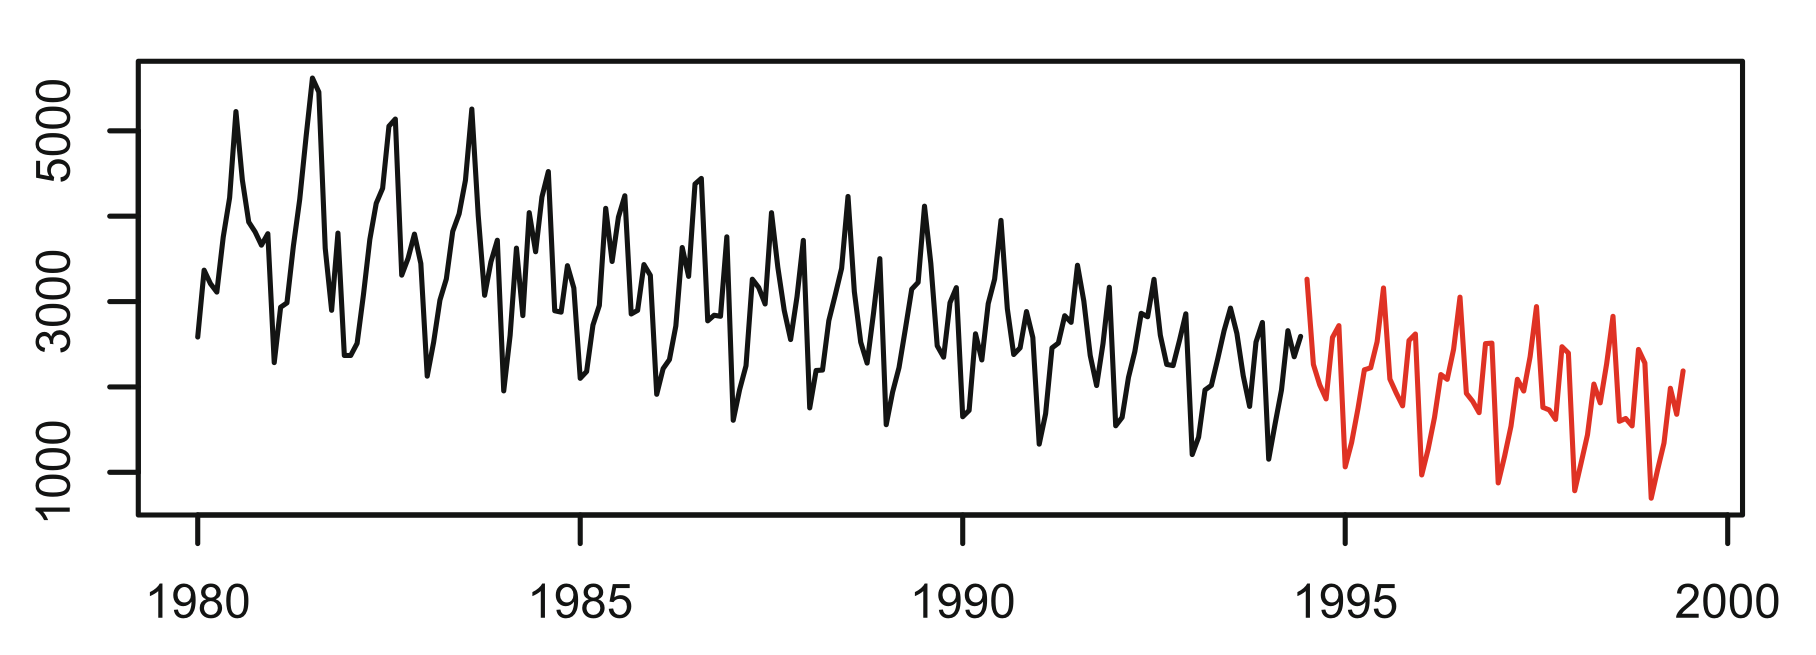
\includegraphics[width=10cm]{forecast.png}
    \end{frame}


    % \begin{frame}
    %     \frametitle{Согласованные сигналы}

        

        

    %     \begin{block}{Пример}
    %         \begin{tabular}{lll}
    %         & $s^{(i)}_j = A_i\cos(\frac{2\pi j}{T_i})$ & $s^{(i)}_j = A_i\exp(j\lambda_i)$ \\
    %         Согласованные:  & $T_1 = T_2 \neq 2$ & $\lambda_1 = \lambda_2$
    %         \\
    %         Несогласованные:& $2 \neq T_1 \neq T_2 \neq 2$ & $\lambda_1 \neq \lambda_2$
    %         \end{tabular}
    %     \end{block}        
    % \end{frame}

    \begin{frame}
        \frametitle{Численные эксперименты}
        
        \begin{block}{Гипотеза}
            Если сигналы рядов согласованны и шум второго небольшой, то ряд $F_2$ --- поддерживающий. 
        \end{block}

        \begin{block}{Вопрос}
            На сколько можно исказить сигнал второго ряда, прежде чем он перестанет быть поддерживающим?
        \end{block}

        Шаблоны рядов в экспериментах:
        \begin{columns}
            \begin{column}{0.5\textwidth}
                \begin{enumerate}
                    \item $s^{(i)}_j = \exp(j\lambda_i)$
                    \item $s^{(i)}_j = \cos(\frac{2\pi j}{12})\exp(j\lambda_i)$
                    \item $s^{(i)}_j = \cos(\frac{2\pi j}{T_i})$
                    \item $s^{(i)}_j = \cos(\frac{2\pi j}{12}) + \exp(j\lambda_i)$
                \end{enumerate}
            \end{column}
            \begin{column}{0.5\textwidth}
                Шумы $\mathsf{R_1, R_2}$ --- независимые белые гауссовские шумы со средними, равными 0, и дисперсиями $\sigma_1^2, \sigma_2^2$, соответственно.
            \end{column}
        \end{columns} 
                
    \end{frame}

    \begin{frame}
        \frametitle{Планы}
        \begin{itemize}
            \item Как по структуре рядов понять согласованность?
            \item Что если ранги рядов разные?
        \end{itemize}
    \end{frame}
\end{document}